\section{Durchführung}
\label{sec:Durchführung}

\subsection{Aufbau}
\begin{figure}
    \centering
    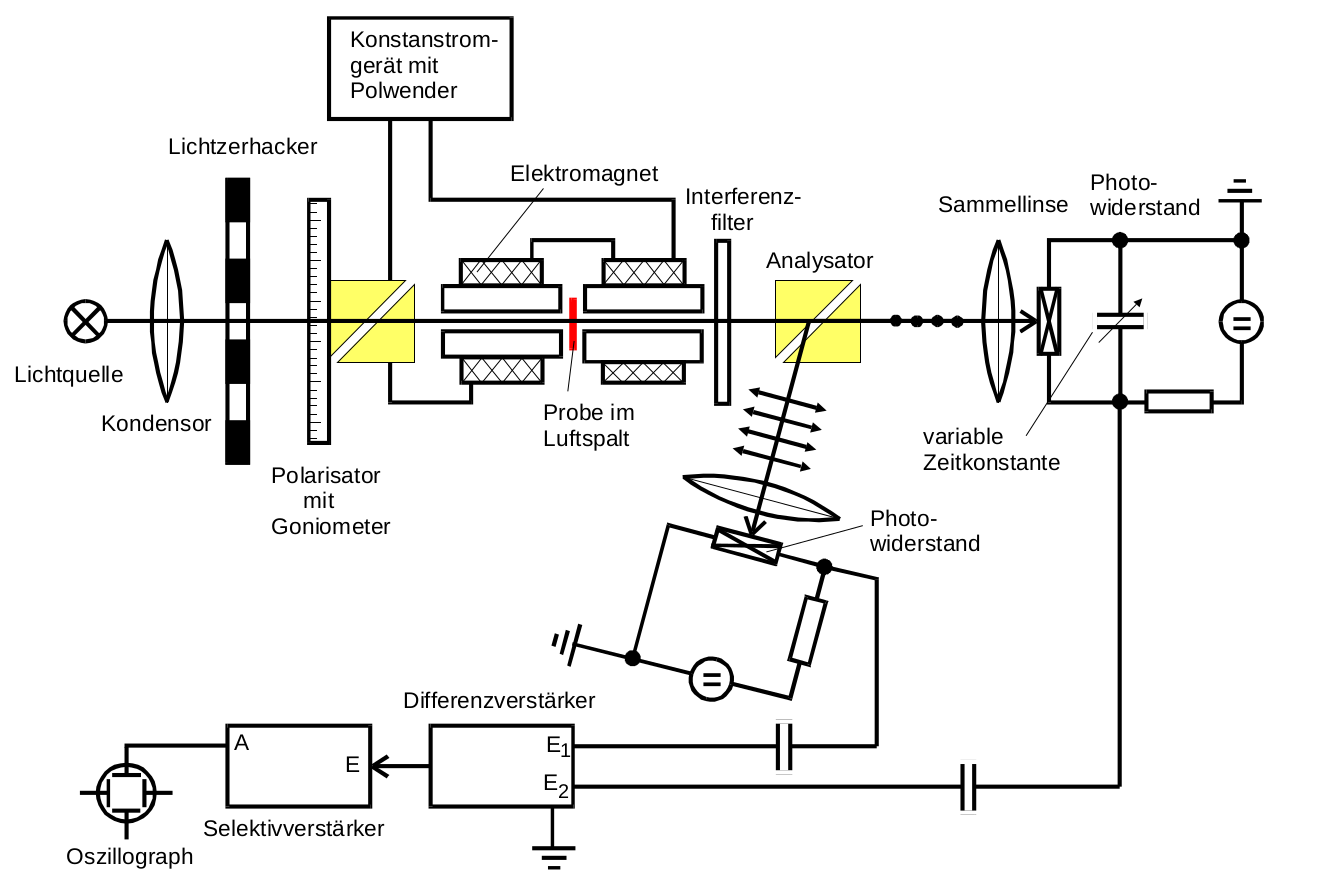
\includegraphics[width=.9\textwidth]{Bilder/Aufbau.png}
    \caption{Schematische Darstellung des Versuchaufbaus. \cite{V46}}
    \label{fig:aufbau}
\end{figure}


Es wird ein Aufbau gemäß Abbildung \ref{fig:aufbau} verwendet. 
Die hier verwendeten Halbleiter bestehen aus GaAs. 
Damit sind sie im infraroten Bereich transparent.
Deshalb wird zur Lichterzeugung eine Halogen-Lampe ($\SI{12}{\volt}$; $\SI{50}{\watt}$) verwendet, welche überwiegend im infraroten Spektrum emittiert.
Nach Emission tritt das Licht durch einen drehbaren Polarisationsfilter, wodurch sich die Polarisationsebene kontrolliert drehen lässt.
Daraufhin durchtritt das Licht die Probe.
Diese befindet sich im Zentrum zweier Spulen, mit denen sich das benötigte Magnetfeld erzeugen lässt.
Folgend wird das Licht mit jeweiligen Interferenzfiltern monochromatisiert.
Zum eigentlichen Messen der Faraday Rotation wird eine Kombination aus einem Wollaston Prisma und zwei Photodetektoren, welche ihr Signal an einen Differenzverstärker weiterleiten.
Der Aufbau ist so kalibriert, sodass bei fehlender Probe der Lichtstrahl zu gleichen Teilen auf die beiden Photodetektoren trifft.
Dies wird dadurch erreicht, da die Polarisationsebene genau digonal zu den beiden Hauptachsen des Wollaston Prismas verläuft.
Dadurch ist die von den jeweiligen Photodetektoren gemessene Lichtintensität identisch.
Findet nun Faraday Rotation statt, messen die Photodetektoren unterschiedliche Intensitäten und es kommt zu einer Differenz.
Diese Methode hat den Vorteil, dass konstanter Untergrund, wie das Umgebungslicht, in der Differenz verschwindet.
Um diese Untergrundtrennung zu optimieren, wird eine Kombination aus einem Lichtzerhacker und einem Selektivverstärker verwendet.
Zu Anfang des Lichtweges wird der Strahl zu bekannter Frequenz in Pulse gestückelt.
Der Selektivverstärker wird auf diese Frequenz eingestellt. 
So lässt sich mit hoher Genauigkeit eine Änderung der Differenz aufzeichnen.
Der Output des Selektivverstärkers wird in ein Oszillokop geführt.
Auf dem Oszillokop ist nun eine sinusoidale Schwingung zu beobachten.


\subsection{Justage}
Es soll sichergestellt werden, dass das Licht in möglichst hoher Intensität auf die Photodetektoren trifft.
Dazu wird das Wollaston Prisma und ein Photodetektor passend verschoben.
Daraufhin wird die Frequenz des Zerhackers mit der des Selektivverstärker abgestimmt.

\subsection{Durchführung}
\label{subsec:Durchfuehrung}
Es wird eine Probe aus GaAs in die vorgesehene Lücke in die Spulen geschoben. 
Dahinter wird ein Polarisationsfilter in den Strahlengang gesetzt.
Bei maximalen Magnetfeld wird der drehbare Polarisationsfilter so lange gedreht, sodass das Signal auf dem Oszillokop minimal wird.
Der Winkel wird notiert, dass Magnetfeld umgepolt und der Polarisationsfilter wird wieder bis zum beobachtbaren Minimum gedreht.
Dieser Vorgang wird mit neun verschiedenen Polarisationsfiltern und damit neun verschiedenen Wellenlängen durchgeführt.
Um die effektive Masse der Leitungselektronen von der der Löcher zu unterscheiden, wird die Faraday Rotation zweimal mit einer n-dotierten GaAs-Probe und einmal mit einer reinen GaAs-Probe vermessen.
Die Vermessung zweier n-dotierter Proben dient der Erhöhung der statistischen Sicherheit.
Schließlich wird die Magnetfeldstärke am Ort der Probe gemessen, welche während der Messungen gewirkt hat.
%Was wurde gemessen bzw. welche Größen wurden variiert?